\documentclass[a4paper]{iacas}% insert '[draft]' option to show overfull boxes

\usepackage{hyperref}% embedding hyperlinks [must be loaded after dropping]
\usepackage{amsmath}
\usepackage{amssymb}
\usepackage{soul,color}
\usepackage{threeparttable}% tables with footnotes
\usepackage{dcolumn}% decimal-aligned tabular math columns
\newcolumntype{d}{D{.}{.}{-1}}
\usepackage{graphicx}
\usepackage{caption}
\usepackage{subfig}
\usepackage{multirow}

\title{Computational Fluid Dynamics Modeling of Cathodic Arc Jet in Stationary Atmospheric Pressure Gas}

\author{%
	Anton Ronis\thanks{Gradute Student. E-mail: ro@tx.technion.ac.il}
	\ and
	Igal Kronhaus\thanks{Assistant Professor. E-mail: kronhaus@technion.ac.il}\\
	{\normalsize\itshape
		Faculty of Aerospace Engineering, Technion, Haifa,
		3200003, Israel}
}

% define some commands to maintain consistency
\newcommand{\pkg}[1]{\texttt{#1}}
\newcommand{\cls}[1]{\textsf{#1}}
\newcommand{\file}[1]{\texttt{#1}}

\begin{document}
	
	\maketitle
	
	\begin{abstract}
		In this paper a computational fluid dynamic (CFD) model of the cathodic arc jet is developed. The CFD simulation is based on an incompressible solver modified with an external body force representing the ion-neutral momentum transfer in the region of plasma-gas interaction.
		The flow properties -- pressure and velocity are qualitatively analyzed in different periods of simulation time. 
		The CFD jet model of the CAJ predicts the experimentally observed pressure front velocity profile. The compatibility of the pressure front velocity profile with the Taylor-Sedov blast model was validated. This simplified empirical model can be used to simulate the CAJ even without modeling the plasma explicitly, greatly reducing the computation requirements.
		 
	\end{abstract}

\section{Introduction}
Active manipulation of flows is an important area of aeronautical research \cite{GADEL}. One prominent example is the use of flow manipulation to reduce drag by delaying and/or eliminating separation zones \cite{SIMPSON}. The literature provides several examples of flow-control devices including: synthetic jets, bleed/suction and plasma actuators.
In contrary to other actuators, plasma actuators can operate on the flow by three different mechanisms \cite{FLOWCTRL}: momentum, shock and chemical effects. Momentum effects induce near surface flow velocities. Shock effects induce very high local gas pressure and temperature gradients in the background gas. Chemical effects introduce new species, such as ions, electrons, and excited particles into the flow field. The most studied plasma actuator configuration is the dielectric barrier discharge (DBD) which is capable of inducing $\sim10$ $m/s$ flows \cite{FLOWCTRL,KOK,WHALLEY,MOREAU}, too low to be effective at high subsonic regimes.

In a recent study \cite{KR}, cathodic arcs operating at atmospheric pressure environment were shown to produce fast jets of gas. This so called cathodic arc jet (CAJ) induces a local flow field velocities of $\ge$ 100 $m/s$ (see Fig. \ref{fig:CAJ}). The jet direction was also shown to be controlled by the application of an external magnetic field. A physical model of the CAJ was developed in a recent paper \cite{KRClose}, relating the cathode and background gas properties to the observed CAJ. Further results suggest the possibility of using the CAJ as a flow-control device for external subsonic flows\cite{KRFar}.

In this paper a computational fluid dynamic (CFD) model of the CAJ is developed. A comparison with available measurement data of the spatial distribution of flow parameters is made. The goal is to examine if the main mechanism of CAJ formation is ion-gas momentum transfer collisions.

\begin{figure}
	\centering
	\includegraphics[width=0.59\textwidth]{CAJ_highres.png}
	\caption{Schlieren images of the cathodic arc jet in air. The luminous plasma shows white. The pressure front is indicated by a thick gray boundary around the heated gas. Time is counted from the moment of ignition. Reproduced from \cite{KR}.}
	\label{fig:CAJ}
\end{figure}

%The numerical solution is carried out using a modified \texttt{OpenFOAM} \cite{OPENFOAM} open source toolbox solver, \texttt{forcedIcoFoam} \cite{NS}. The \texttt{forcedIcoFoam} is a pressure based solver for transient incompressible flows modified to include an external force field acting on the flow.
%
%The numerical approach is based on the assumption that the CAJ effect on the background gas can be simulated by an application of acceleration field which causes the gas to reach the velocities obtained in the \cite{KR}. Therefore the jet simulation corresponds to a hot gas expansion at a subsonic speed. Following measurement data \cite{KRClose}, the acceleration field was adjusted to yield a velocity of $500~ m/s$.
%
%The flow properties -- pressure and velocity qualitatively analyzed in different periods of simulation time. Sampling the pressure front position and static values, caused by the jet expansion with respect to time allows one to compare the results obtained from the simulation with \emph{Taylor-Sedov} blast model \cite{TAYLOR,SEDOV}  .
%The pressure front position and velocity obtained in a simulation are visualized in Fig. \ref{fig:model_position} and Fig. \ref{fig:model_velocity}, respectively. The results correspond well with the measured data in \cite{KR}.
%
%The CFD jet model of the CAJ predicts well the observed phenomenons from \cite{KR} -- \emph{i.e.} forming of an initial cylindrical expansion zone at $1~\mu s$, steady conditions in the jet area after around $t = 100~\mu s$, and compatibility with the \emph{Taylor-Sedov} blast model pressure front position and velocity, with respect to time and distance, respectively. Modeling the CAJ as a jet results in some deficiencies -- mainly the addition of mass to the background gas domain and the generation of vortices caused by the flow expansion at the inlet edge. These deficiencies are notable in the local jet domain and must be accounted for in the final CFD model of the CAJ. 
%
%

\section{Physical Model}\label{sec:physical_model}
The schlieren time sequence images shown in Fig. \ref{fig:CAJ} allow us to postulate the following process for the formation of the CAJ:
\begin{enumerate}
	\item Plasma formation in a bounded region
	\item Pressure front expansion
	\item CAJ plume gas-dynamic expansion towards the background gas
\end{enumerate}

In the first event a small yet energized volume of plasma particles is generated. A pressure boundary is formed with a radius size determined by the cathode parameters, discharge current and the background gas pressure \cite{boxman1990momentum}.
Subsequently, the second event begins with an expansion of the pressure front. This expansion is followed by the formation of a jet caused by a momentum and energy transfer of the plasma particles to the gas. It is seen that after the initial CAJ expansion certain steady-state conditions are met in the luminous jet region. 

The evolution of the initial pressure wave due to the formation of plasma can be modeled using a Taylor-Sedov blast wave model \cite{TAYLOR,SEDOV}: 

\begin{eqnarray}\label{eqn:taylor_sedov}
r^5 t^{-2} &=& \mathrm{constant}
\end{eqnarray}

\noindent The pressure wave visualized as dark boundary in Fig. \ref{fig:CAJ}, initially starts with a sonic velocity at the plasma boundary, and quickly decays at $\approx 10~\mathrm{mm}$. Following the pressure wave expansion, the CAJ, shown as a luminous jet in Fig. \ref{fig:CAJ}, is formed at the plasma-gas boundary. Close to the plasma-gas boundary, the CAJ is assumed to follow the initial pressure wave expansion velocity. The physical model developed in \cite{KRClose} suggest that the CAJ is formed mainly due to momentum transfer from ions to the gas.


The force exerted on the plasma particles can be written as (similar to the derivation in \cite{boxman1990momentum}):

\begin{eqnarray}\label{eqn:plasma_force}
	F_i &= &\frac{M_i V_i f}{Z e} I_d
\end{eqnarray}

\noindent where $M_i$ is the ion mass, $V_i$ is the ion velocity, $f$ is the ion current fraction, $Z$ is the charge state, $I_d$ is the discharge current magnitude and $e$ is the electron charge.
Assuming an equilibrium between the plasma and gas induced forces, Eq. \eqref{eqn:plasma_force} can be used to find the area $A$ for which the equilibrium is achieved:

\begin{eqnarray}\label{eqn:rel_equiv_force}
	F_g & = & F_i \\
	p A & = & \frac{M_i V_i f}{Z e} I_d\\
	A & = & \frac{M_i V_i f}{Z e} \frac{1}{p} I_d
\end{eqnarray}

\noindent where $F_g$ and $F_i$ are the background gas pressure force and the ion momentum transfer force, respectively. Assuming hemi-spherical distribution of the gas pressure force on the plasma, i.e $A = \pi r^2$, the following expression is obtained for the radius, $r$:

\begin{eqnarray}
\label{eqn:rad_equiv_force}
	r & = & \mathcal{C}\sqrt{I_d}
\end{eqnarray}


\noindent where $\mathcal{C} = \sqrt{\frac{1}{\pi}\frac{M_i V_i f}{Z e}\frac{1}{p}}$ is a constant defined by the cathode and experimental parameters. Eq. \eqref{eqn:rad_equiv_force} relates the boundary radius $r$ to the discharge current, $I_d$. Results for the given parameters in the experiments \cite{KR,KRClose} are shown in Table~\ref{t:radii}.
\begin{table}[h]
	\begin{center}
		\begin{threeparttable}
			\caption{Calculated CAJ boundary radius}
			\label{t:radii}
			\begin{tabular}{l|c|c}
				Parameter & Case 1 & Case 2\\ \hline
				$I_d~[A]$& 230 & 40\\
				$p~\mathrm{[Pa]}$ & $101 \times 10^3 $ & $101 \times 10^3 $ \\
				$T~\mathrm{[K]}$	& $870$ & $870$ \\
				$\gamma$ & $1.365$ & $1.365$ \\ 
				$\mathrm{M}$	& $0.856$ & $0.856$ \\
				$M_i~\mathrm{[kg]}$ & $1.055 \times 10^{-25} $ & $1.055 \times 10^{-25} $  \\
				$V_i~\mathrm{[m/s]}$ 	& $12.5 \times 10^3 $ & $12.5 \times 10^3 $  \\
				$f$ 	& $0.08 $ & $0.08 $ \\
				$Z$	& $1.8 $ & $1.8 $ \\
				$\mathrm{M}$	& $0.856$ & $0.856$ \\
				$r~\mathrm{[mm]}$ 	& 0.51& 0.21
			\end{tabular}
		\end{threeparttable}
	\end{center}
\end{table}
As Table~\ref{t:radii} shows the plasma-gas boundary is $\lesssim 0.5~\mathrm{mm}$.

In steady state conditions at the plasma-gas boundary, assuming a constant discharge current $I_d$, we can express the exerted force on the gas with respect to velocity as:

\begin{align}\label{eqn:force_mass_flux}
	F_i & = F_g = \dot{m} V_g
\end{align}

\noindent where $V_g$ is the gas velocity at the plasma-gas boundary. Substituting the mass flow rate $\dot{m}$ for $\rho V_g A_{o}$ -- where $A_{o}$ represents a circular cross section through which the jet flows and $\rho$ is the fluid density, yields:

\begin{eqnarray}\label{eqn:force_density}
F_g &=& \rho V^2_g A_{o}
\end{eqnarray}

\noindent As the boundary radius is defined by the equivalence between the pressure force and the ion force, 
Eq. \eqref{eqn:force_density} thus yields:

\begin{eqnarray}\label{eqn:force_gas_equal}
p A &=& \rho V^2_g A_{o}
\end{eqnarray}

The CAJ initial temperature can be estimated by substituting the areas $A$ and $A_o$: 

\begin{eqnarray}\label{eqn:force_gas_ratio}
p \cdot \pi r^2 &=& \rho V^2_g \cdot \pi r^2 \\
\frac{p}{\rho} &=& V^2_g
\end{eqnarray}

Using the state equation for an ideal gas, $p = \rho RT$, we get:

\begin{eqnarray}\label{eqn:force_gas_temperature}
	T &=& \frac{V^2_g}{R}
\end{eqnarray}

\noindent where $T$ is the temperature and $R$ is the specific gas constant. Eq. \eqref{eqn:force_gas_temperature} relates the gas temperature to the jet velocity. Substituting $R = 287~J\cdot kg^{-1} K^{-1}$ and applying the gas velocity measured in \cite{KRClose} $V_g = 500~$m/s (Case 2 in Table~\ref{t:radii}) a gas temperature value of $\approx 870~\mathrm{K}$ is obtained. From Eq. \eqref{eqn:force_gas_temperature} we can express the Mach number at the boundary, as:

\begin{eqnarray}
	\mathrm{M} &=& \frac{V_g}{a} \\
	 &\approx& \frac{\sqrt{RT}}{\sqrt{\gamma R T}}\\\label{eqn:mach}
	 &=& \sqrt{\frac{1}{\gamma}}
\end{eqnarray}

\noindent where $a$ is the speed of sound. For most cases, the heat capacity ratio $\gamma \geq 1$. %Specifically for ideal air at $1000^o~C$ $\gamma = 1.365$ -- We can therefore conclude that the boundary Mach is $\mathrm{M} = 0.856$. 
Values of Mach number and temperature are summarized in Table~\ref{t:radii} using dry air values. The Mach number is therefore smaller than 1.

\clearpage 

\section{Numerical Model}

The CFD numerical approach is derived from the assumption that the CAJ is predominantly influenced by gas dynamics effects after being accelerated by momentum transfer collisions between ions and gas inside the plasma-gas boundary region, and therefore can be simulated by the application of an acceleration field which causes the gas to reach the velocities measured in \cite{KR}. This corresponds to adding a body force acceleration to the incompressible Navier-Stokes momentum equations:

\begin{eqnarray}
\label{eqn:NS-Force}
\frac{\partial \boldsymbol{u}}{\partial t} + (\boldsymbol{u} \cdot \nabla)\boldsymbol{u} &=& -\frac{1}{\rho}\nabla p + \frac{\mu}{\rho} \nabla^2 \boldsymbol{u} + \boldsymbol{F_b}
\end{eqnarray}

\noindent where $\boldsymbol{u}$ is the flow field velocity and $\boldsymbol{F_b}$ represents the acceleration field.

The numerical solution is carried out using a modified \texttt{OpenFOAM} \cite{OPENFOAM} open source toolbox solver, based on the \texttt{icoFoam} solver. The \texttt{icoFoam} is a pressure based solver for transient incompressible flows which was modified to include an external force field acting on the flow. An incompressible solver was used due to its simplicity and fast calculation time. It is therefore important to note that compressibility effects are not taken into account. The use of an incompressible solver can be justified by the fact that $\mathrm{M} < 1$ at boundary, as described in Section \ref{sec:physical_model}.

The numerical domain consists of 200 $\times$ 300 grid points representing a 15 mm $\times$ 30 mm physical domain. Grid dimensions were obtained by conducting grid size sensitivity runs and analyzing the CAJ profile. The grid density is adjusted at the wall region to yield a maximal cell height of 0.1~mm. 

We simulate the plasma-gas interaction (ions momentum transfer collisions) by assuming a constant acceleration field just upstream the CAJ expansion plume region. The field properties are calculated to correspond with the plasma-gas boundary given in Eq. \eqref{eqn:rad_equiv_force}. Following the observed experimental results shown in Fig.~\ref{fig:CAJ}, the acceleration field was placed at $0  < y \leq 0.5~ \mathrm{mm} $ with a half-width of $0.5~\mathrm{mm}$, centered around $x=0~\mathrm{mm}$. These values correspond to a discharge current of 230 A (Case 1 in Table~\ref{t:radii}).
Following the micrometer resolution CAJ measurement data in \cite{KRClose} (Case 2 in Table~\ref{t:radii}), the acceleration field was adjusted to yield a velocity of $500$ m/s at the boundary $y = 0.5~\mathrm{mm}$. It is assumed that the discharge current and gas pressure affect only the initial plasma-gas boundary location. The effect of increased $I_d$ is increased width. The background gas is stationary, with $p_o = 101\cdot 10^3~\mathrm{Pa}$ and $T_o = 300~\mathrm{K}$.

\section{Results \& Discussion}

The simulation was executed using adaptive time steps with a Courant number $\mathcal{C} \leq 0.1$, for a total simulation time of $t = 500~\mu s$. The solution region of interest includes the CAJ gas dynamic expansion region ($ y > 1~\mathrm{mm} $). The velocity and pressure field spatial distributions, obtained at $ t = 500~\mu s $, are shown in Fig. \ref{fig:velocity_field} and Fig. \ref{fig:pressure_field}, respectively. We observe that the acceleration field results in the formation of a time evolving axisymmetric jet that reaches a quasi-steady-state condition between $1 < y < 10$ mm after $t = 150~\mu s$.
The CFD pressure front position and velocity data are used to produce Fig. \ref{fig:model_velocity} and Fig. \ref{fig:model_position}. Fig. \ref{fig:model_velocity} shows good correspondence between CFD results and the measured data. In Fig. \ref{fig:model_position} good correspondence is obtained between the Taylor-Sedov blast model and the pressure/velocity front velocities obtained in the simulation. The measurement results taken from \cite{KR} diverge near the boundary probaly due to transient effecs and the small number of the data points available.

The pressure front velocity and the CAJ velocity profile evolution are shown in Fig. \ref{fig:model_caj_velocity}. We observe that the velocity profile developed in the CAJ  follows the same trend as the pressure front velocity. However, the CAJ velocity is higher than the pressure front velocity in the entire region. The CAJ axial velocity gradient ($\frac{\mathrm{d}V_y}{\mathrm{d}y}$) is shown in Fig. \ref{fig:model_caj_acceleration}, for several time instances. For each instantaneous moment, we can observe a sharp decrease of the gradient magnitude at a certain distance from the cathode spot. We note that the gradient values converge at a distance of about 6~mm (dotted vertical line). It is interesting to note the correspondence of this location with the termination of the luminous jet in the CAJ observed in Fig. \ref{fig:CAJ}.
\begin{figure}
	\centering
	
	\subfloat[]{
		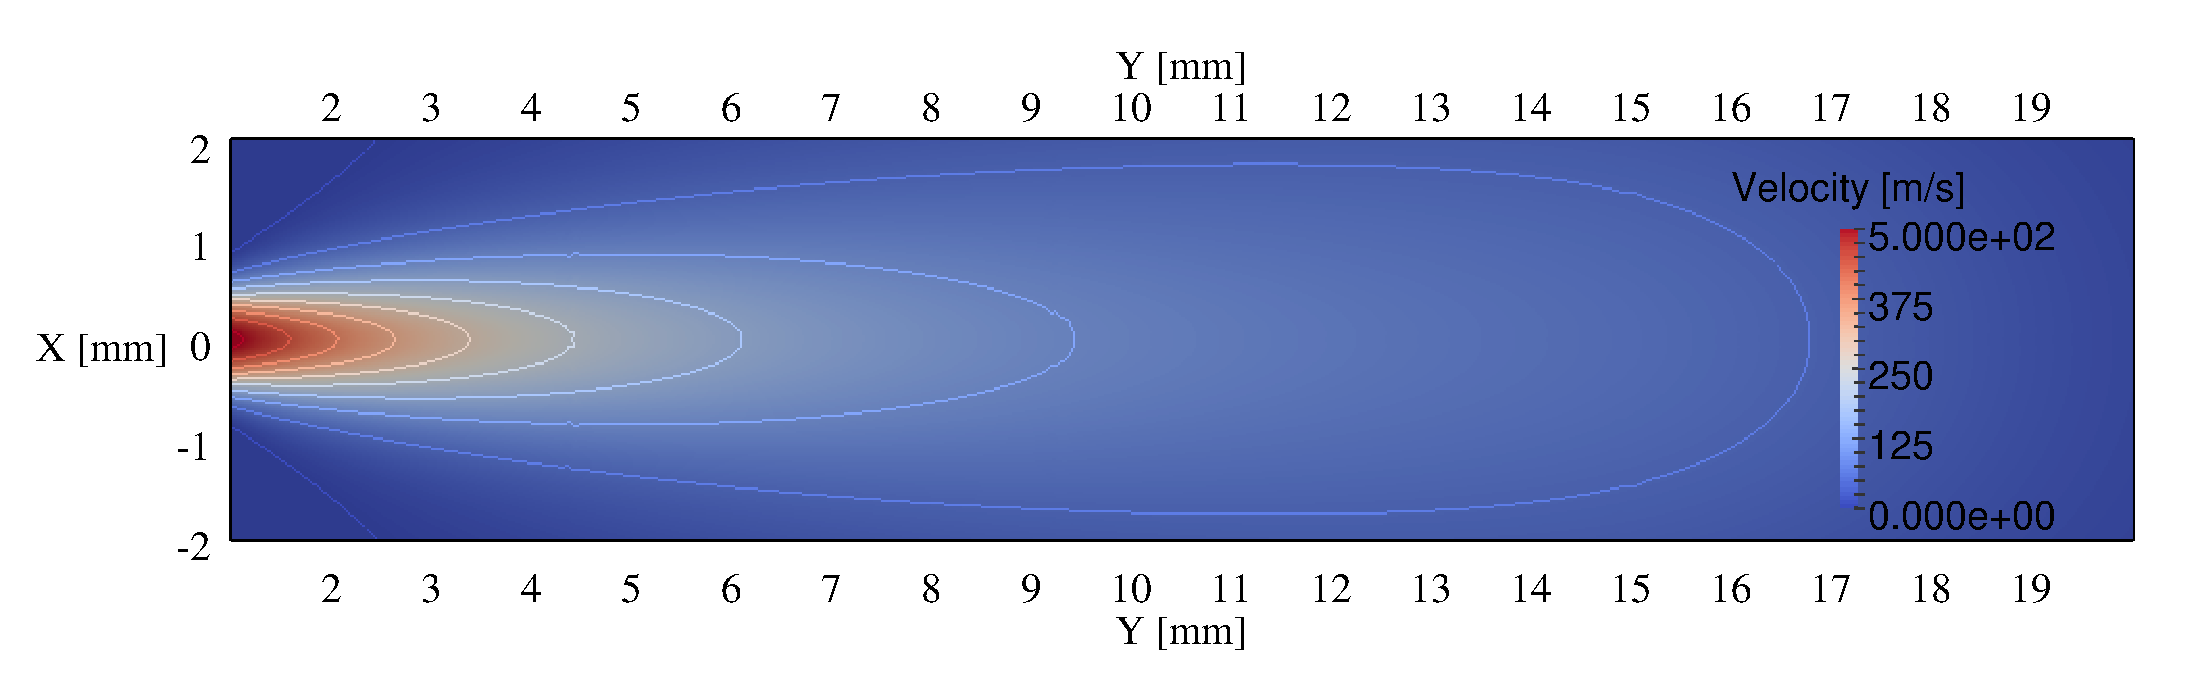
\includegraphics[width=0.86\textwidth]{velocityField}
		\label{fig:velocity_field}
	}
	
	\subfloat[]{
		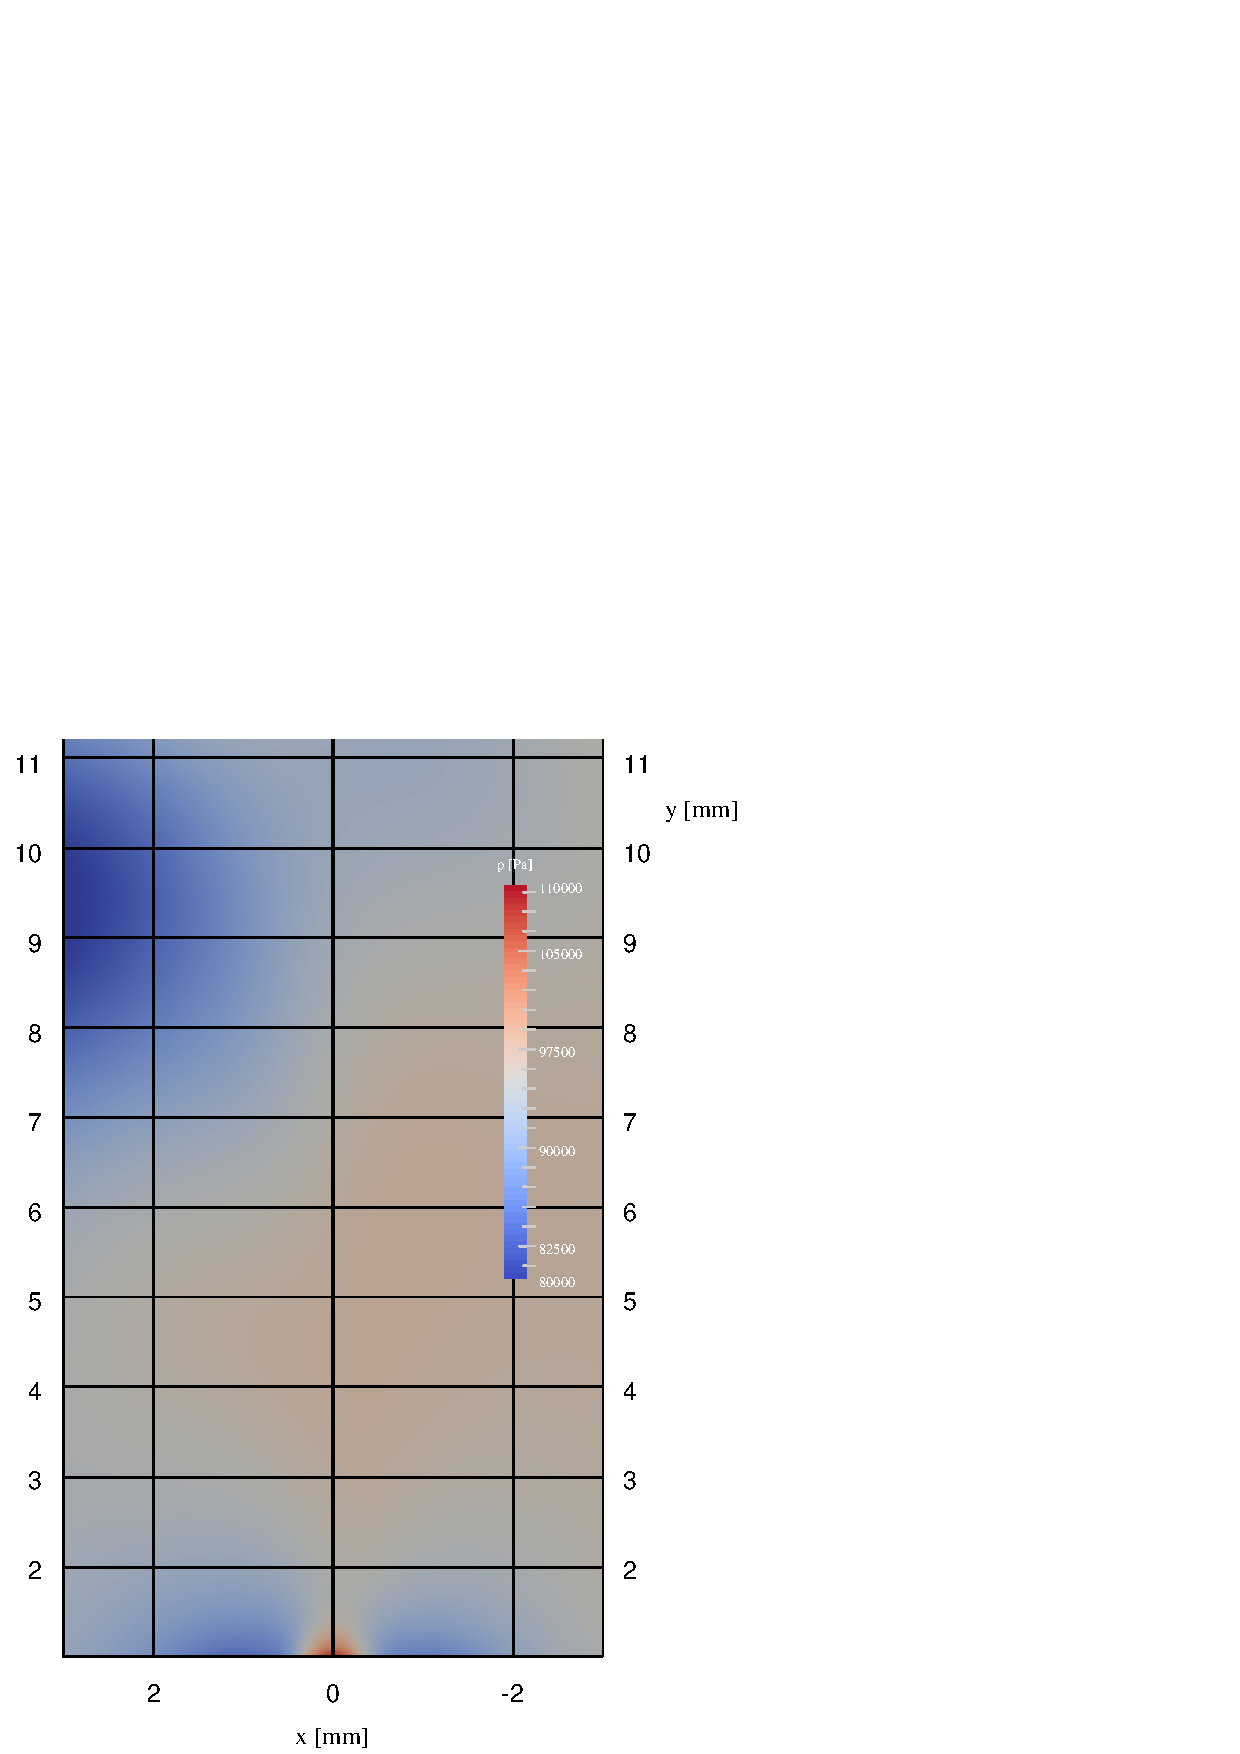
\includegraphics[width=0.86\textwidth]{pressureField}
		\label{fig:pressure_field}
	}
	\caption{(a) Velocity field spatial distribution, $ t = 500~\mu s $; (b) Pressure field spatial distribution, $ t = 500~\mu s $}
\end{figure}
\begin{figure}
		\centering
	\begin{minipage}[t]{0.48\textwidth}
		\centering
		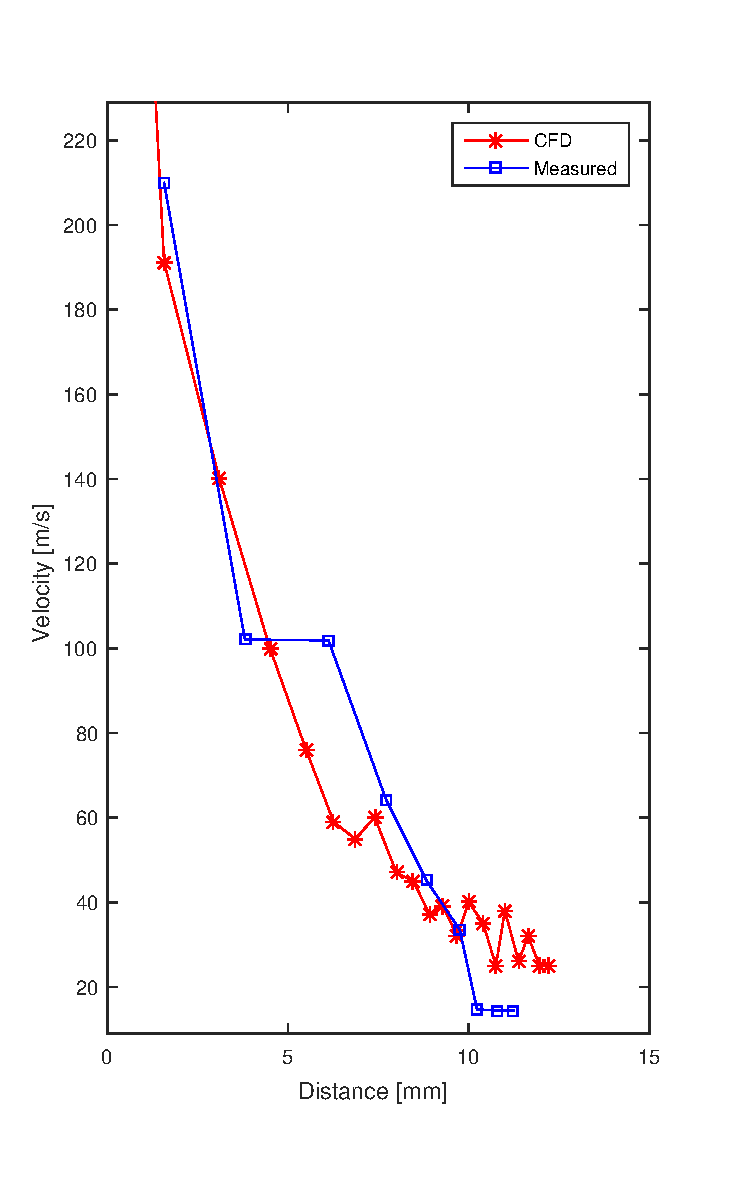
\includegraphics[width=0.8\textwidth]{ModelJetVelocity.eps}
		\caption{The gas pressure front velocity versus position, measured in the direction of the plasma jet (squares) together with the computed CFD velocity of the front (stars). Experiment data reproduced from \cite{KR}.}
		\label{fig:model_velocity}
	\end{minipage}\hfill
	\begin{minipage}[t]{0.48\textwidth}
		\centering
		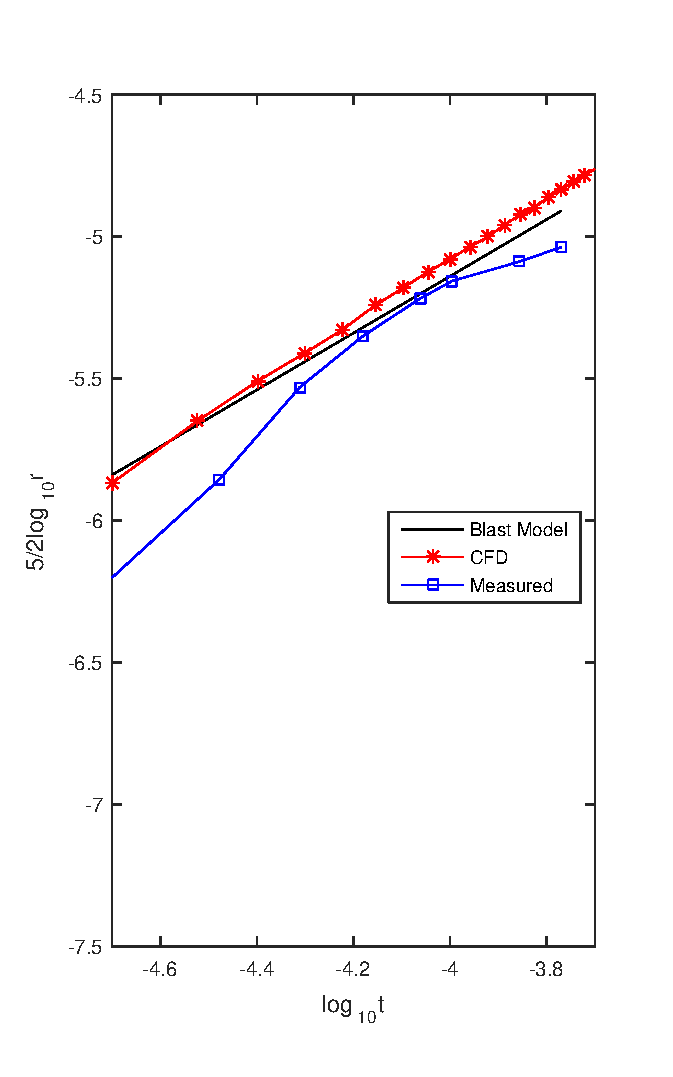
\includegraphics[width=0.8\textwidth]{ModelJetPosition.eps}
		\caption{Time evolution of gas pressure front position (squares - experiment, stars - CFD) together with a linear fit of the blast wave model (black line)}
		\label{fig:model_position}
	\end{minipage}
\end{figure}
%\begin{figure}
%	\centering
%	\subfloat[Position]{
%
%	}
%	\subfloat[Velocity vs. Position]{
%
%	}
%	\caption{(a) ; (b) }
%	\label{fig:model_blast}
%\end{figure}
\begin{figure}
	\centering
	\includegraphics[width=0.8\textwidth]{Vel_Times.eps}
	\caption{Simulation results of front expansion rate (red squares); Time evolution of the CAJ axial velocity versus axial position for sample times of $10~\mu s$, $50~\mu s$, $100~\mu s$, $150~\mu s$ and $500~\mu s$  (blue line).}
	\label{fig:model_caj_velocity}
\end{figure}
\begin{figure}
	\centering
	\includegraphics[width=0.8\textwidth]{CAJAcceleration.eps}
	\caption{Simulation results of time evolution of the CAJ axial velocity gradient ($\frac{\mathrm{d}V_y}{\mathrm{d}y}$), for sample times of $10~\mu s$, $50~\mu s$, $100~\mu s$, $150~\mu s$ and $500~\mu s$ (blue line); the vertical line (black dotted) indicates the position where the gradient cross at different times. }
	\label{fig:model_caj_acceleration}
\end{figure}
\section{Conclusions}
A CFD model of the cathodic arc jet was developed.
A modified incompressible solver was used to include a region of constant external force, simulating the acceleration of the background gas due to the plasma ions momentum transfer.
The flow properties -- pressure and velocity were qualitatively analyzed in different periods of simulation time. The computed pressure front velocity shows good agreement with previous shclieren measurements of the jet. Although the CAJ velocity was not measured before, the CFD results predict that the CAJ velocity is higher than the pressure front velocity.
We can conclude that ion-neutral momentum transfer occur within the plasma-gas boundary, proving that the CAJ initial velocity is controlled by gas dynamic expansion. 
Future studies will analyze the effects of a cross-flow on the CAJ based on the suggested implementation of the model.

\clearpage
\bibliography{bibtex_database}
\bibliographystyle{iacas}
\end{document}


%%% Local Variables:
%%% mode: latex
%%% TeX-master: t
%%% End:
